
\tab For our group project, we are required to design and implement a program that can create and convert Unified Modelling Language (UML) class diagrams to java stub code. For this we will create a graphical user interface, in which the user will be able to create, delete and modify classes, add relationships between classes and add text labels in a UML class diagram. 

The functionality of the program that we will implement can be split into three general groups: file management, software design and diagram editing. A use case diagram for each of the above groups is provided is provided below. 

\vspace{-10pt}
\begin{center}
	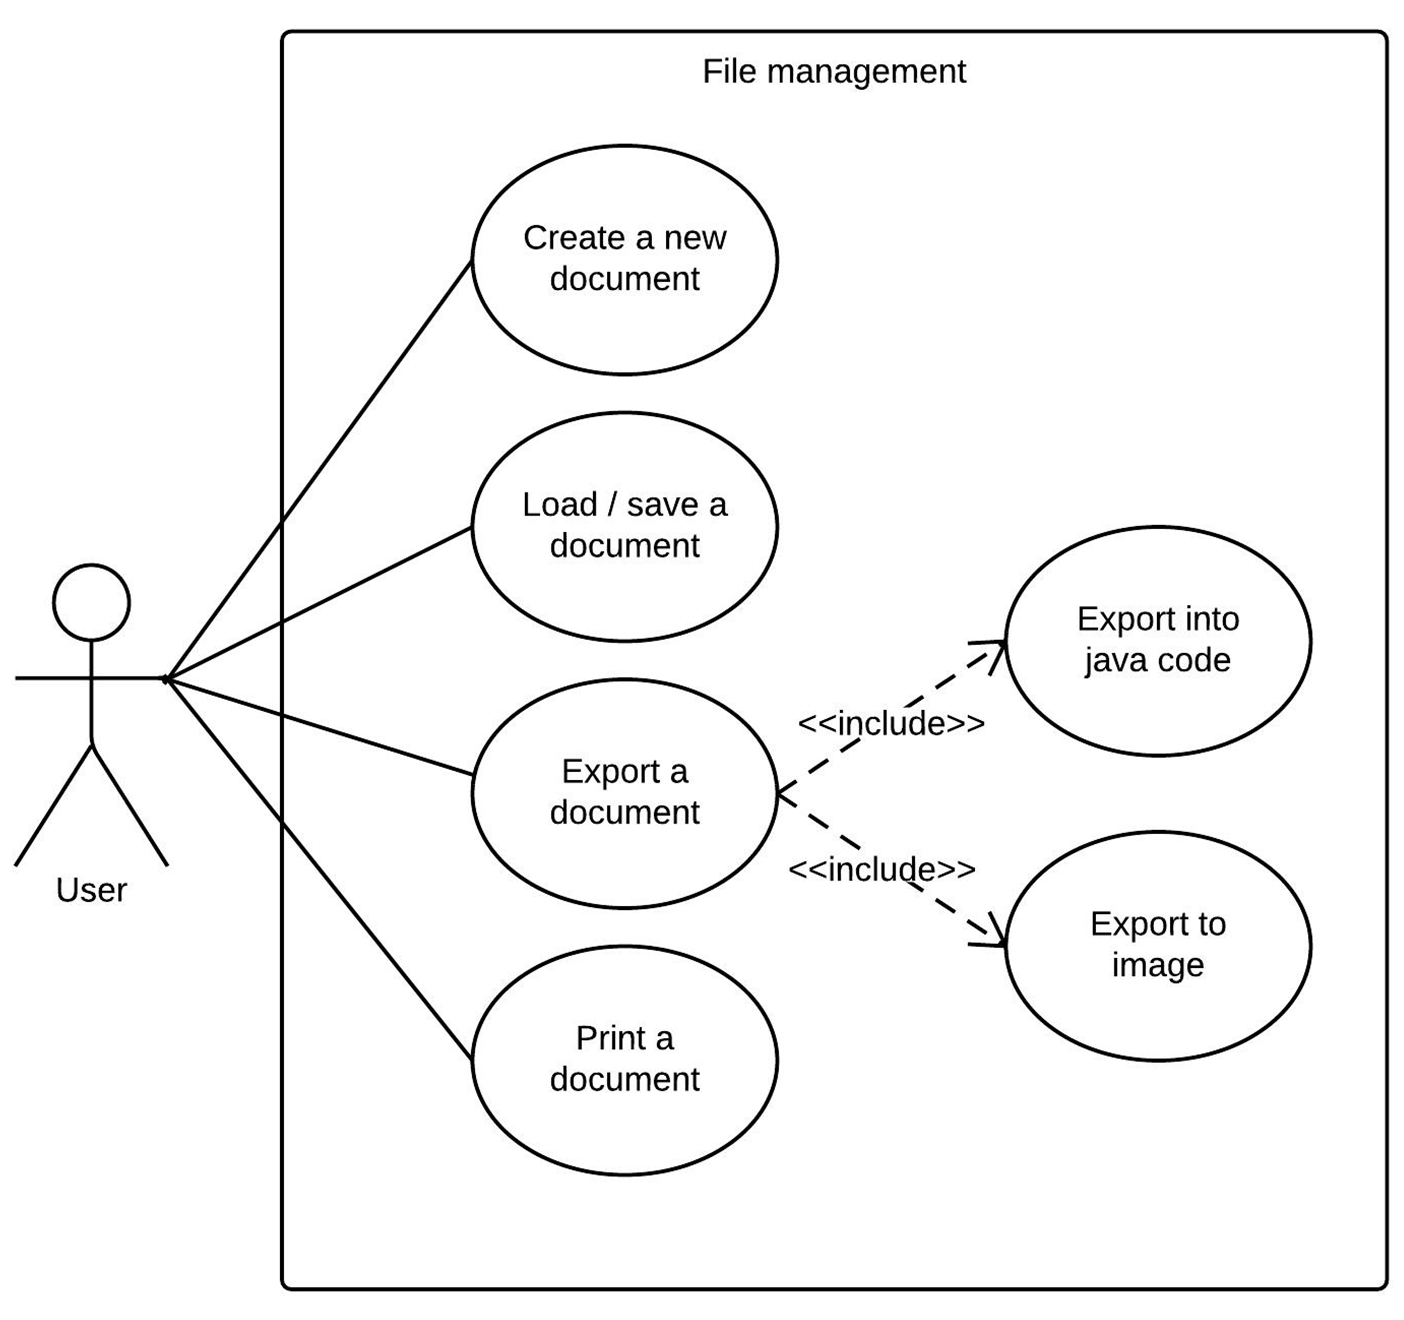
\includegraphics[width=0.45\textwidth]{FileManagementUseCaseDiagram.png}
\end{center}
\vspace{-10pt}

The file management functionality of the program will include the following features: the user will be able to open a new document or load an existing one from a file, as well as save the current document. The program will also be able to export the currently opened class diagram into corresponding .java files containing the user-entered data fields and method stubs. It will also be possible to export a .png, .jpg or .gif image of the diagram canvas that can be easily added to any design documentation. The choice of file or directory relevant to each of these features will be up to the user and will be facilitated by the GUI. An option to print the current diagram will also be implemented.

\vspace{-10pt} 
\begin{center}
	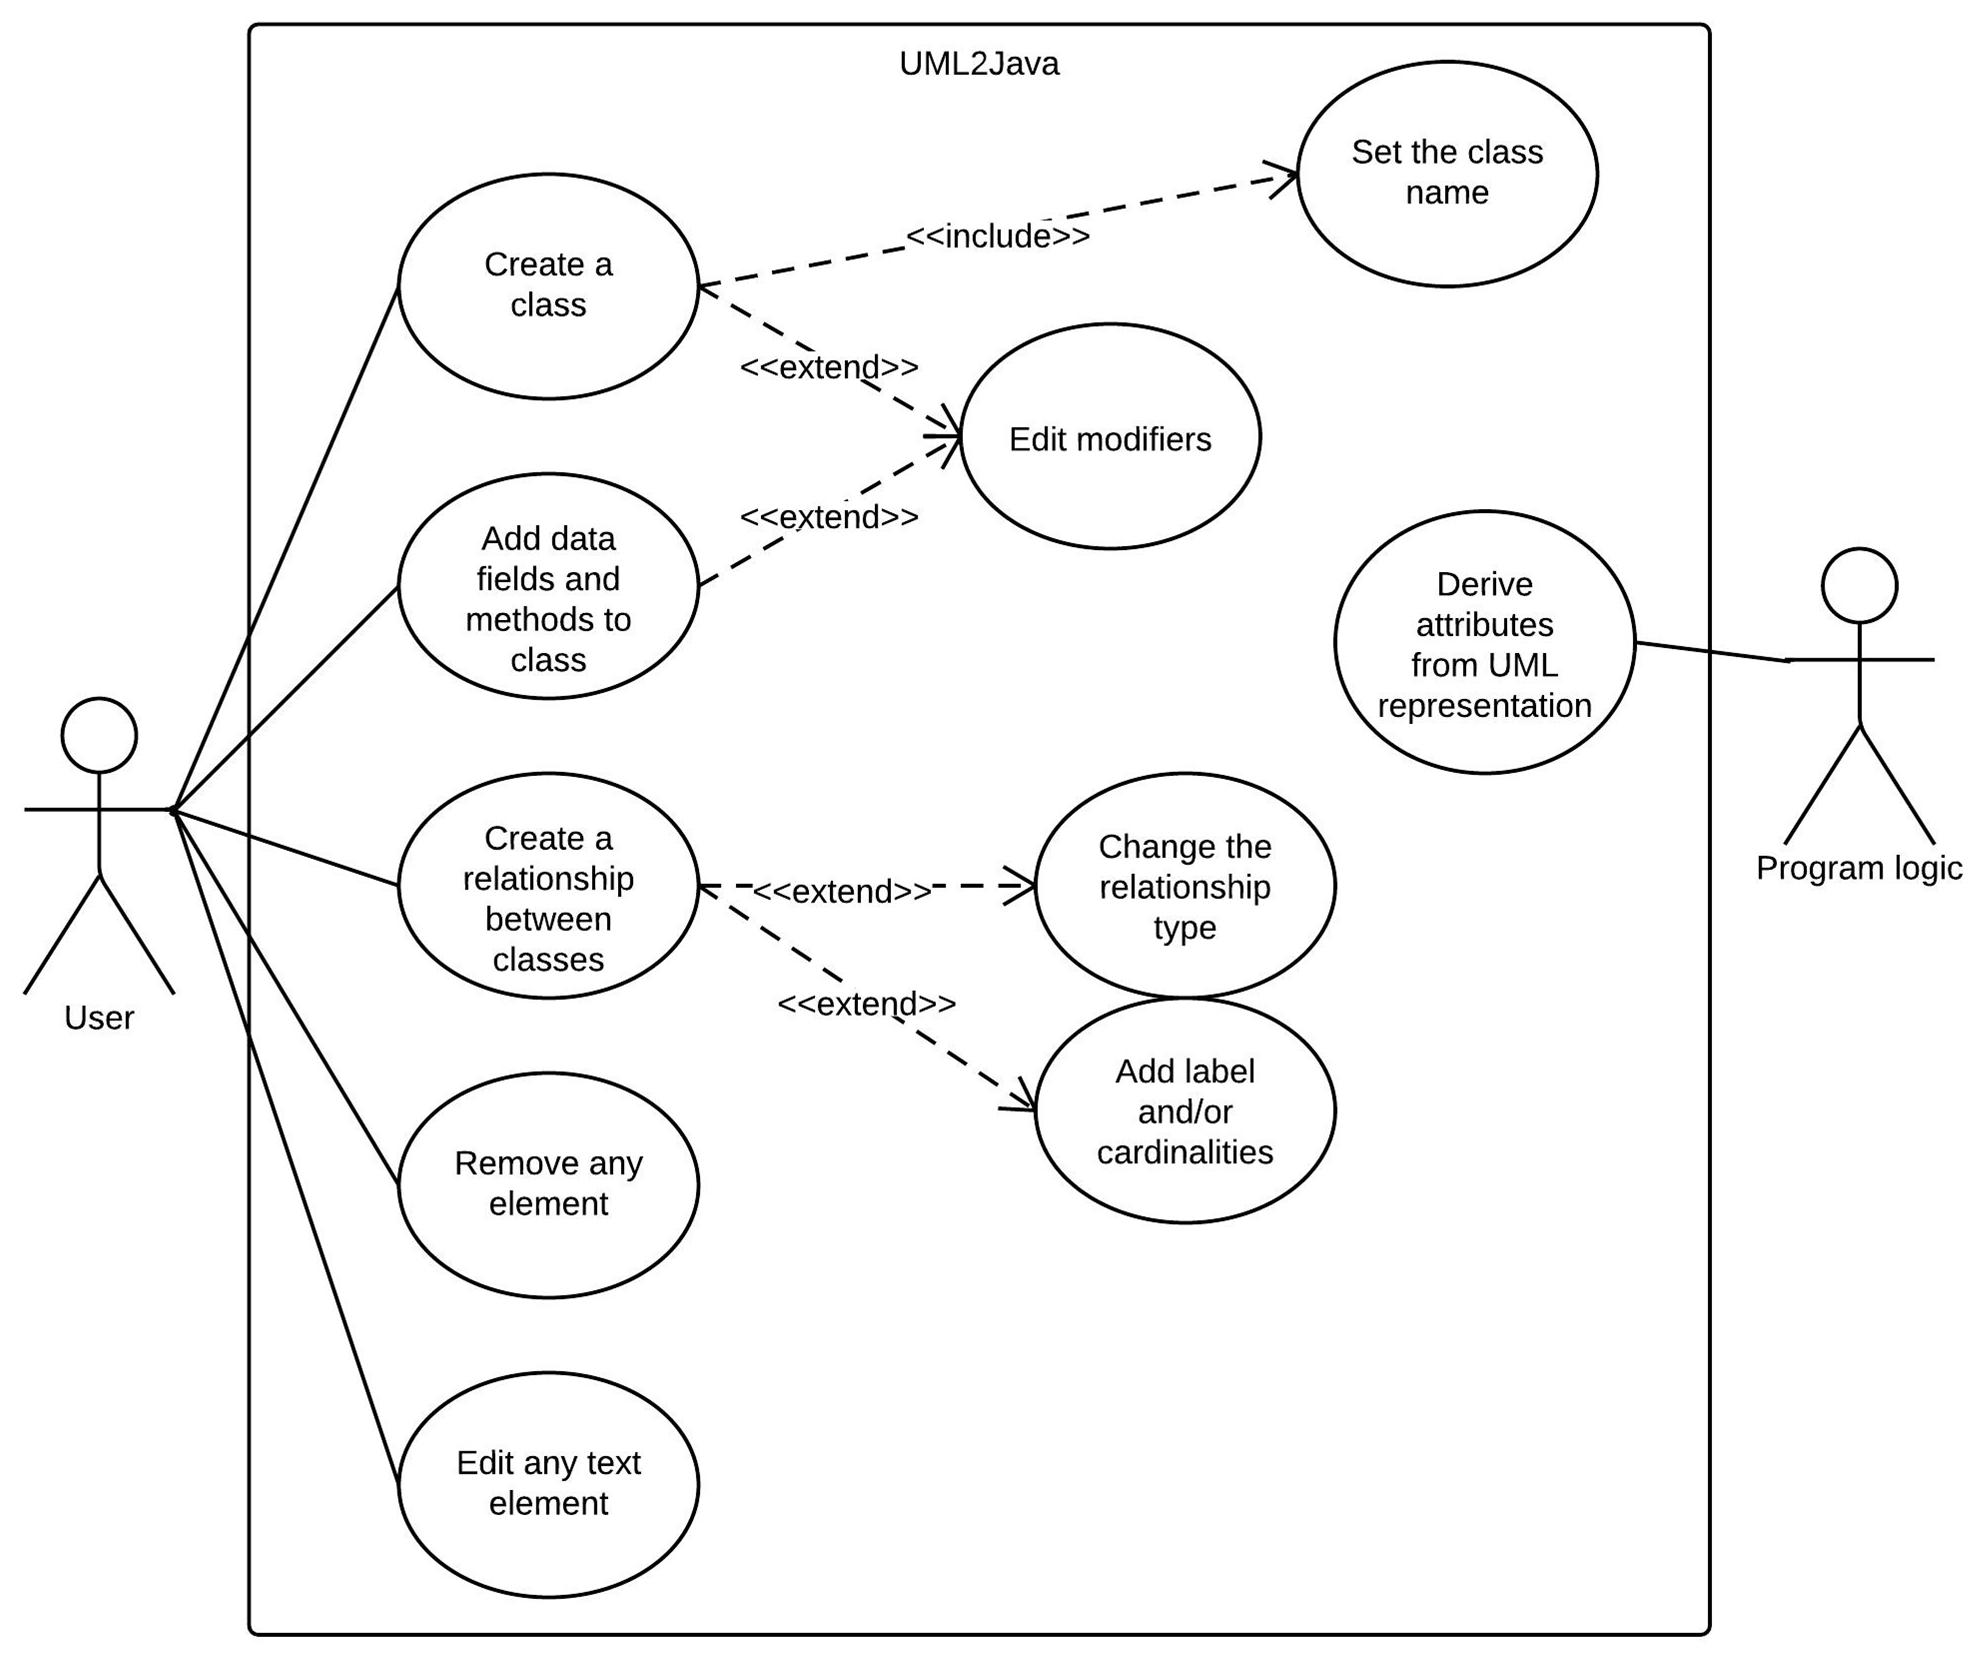
\includegraphics[width=0.65\textwidth]{SoftwareDesignUseCaseDiagram.png}
\end{center}
\vspace{-10pt}

The software design features will include the following: creating a new class, adding data fields and methods to it using standard UML notation from which the program will automatically deduce certain parameters like visibility, type and so on. Modifiers that are not supported by direct UML notation will be accessible through a right-click menu, both for classes and for attributes. The user will be able to add relationships between classes, change their type and add labels and/or cardinalities to them. Any element created this way will be easily editable and removable.

\vspace{-10pt}
\begin{center}
	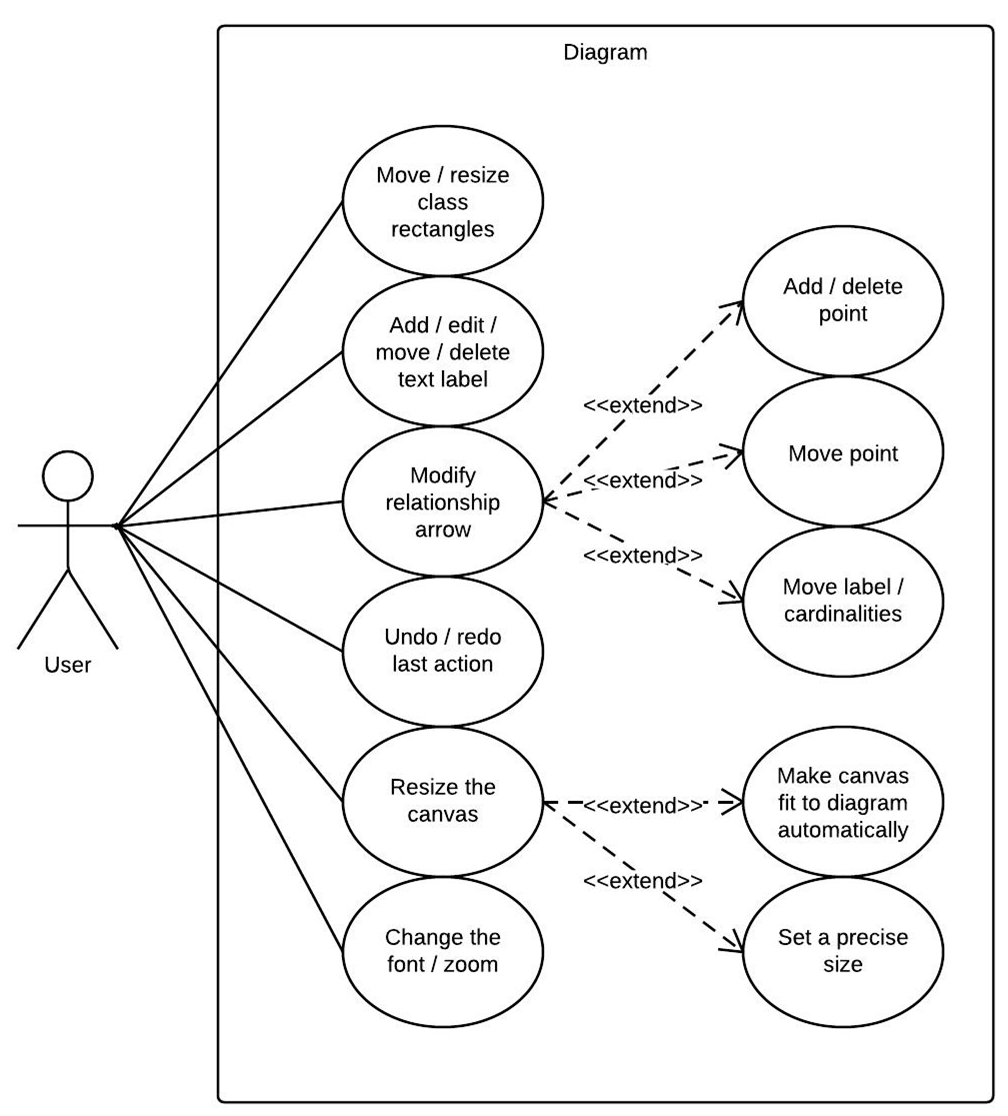
\includegraphics[width=0.5\textwidth]{DiagramUseCase.png}
\end{center}
\vspace{-10pt}

As we are aiming to let the user produce complete UML class diagrams, additional features will be necessary. Class rectangles will be movable and resizable and the user will be able to add text labels to any point on the diagram. Relationships will be highly controllable: moving around points will be possible, as well as adding new points or removing existing ones. The canvas size will be configurable to allow facilitate image export and printing. The user will be able to change the global font used in the diagram and also view the diagram under zoom. We will also attempt to implement an undo / redo facility for user actions.
